\documentclass[border=10pt]{standalone}
\usepackage{pgfplots}
\pgfplotsset{compat=1.18}
\usepgfplotslibrary{fillbetween}
\begin{document}
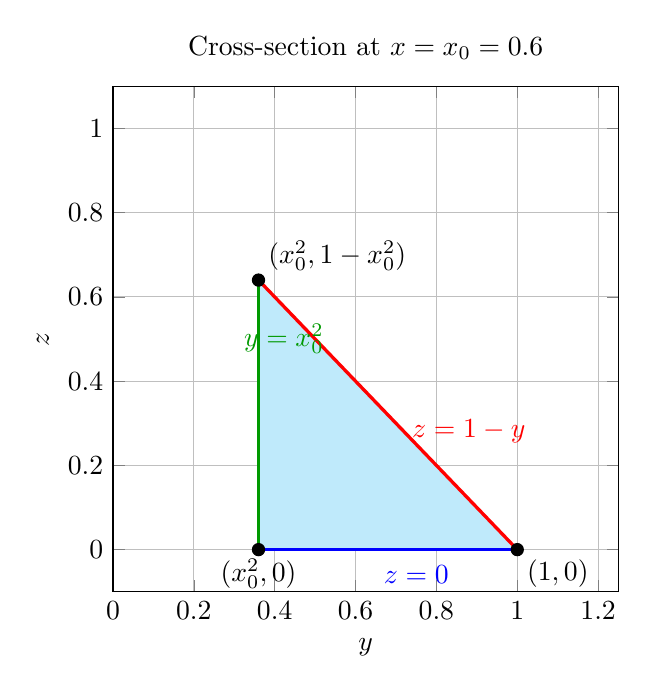
\begin{tikzpicture}
\begin{axis}[
    width=8cm, height=8cm,
    xmin=0, xmax=1.25, ymin=-0.1, ymax=1.1,
    xlabel={$y$}, ylabel={$z$},
    title={Cross-section at $x=x_0=0.6$},
    grid=both, samples=100,
]
\addplot[name path=top, red, very thick, domain=0.36:1] {1-x};
\addplot[name path=bot, blue, very thick, domain=0.36:1] {0};
\addplot[cyan!25] fill between[of=top and bot];
\draw[green!60!black, very thick] (axis cs:0.36,0) -- (axis cs:0.36,0.64);
\node[red]   at (axis cs:0.88,0.28) {$z=1-y$};
\node[blue]  at (axis cs:0.75,-0.06) {$z=0$};
\node[green!60!black, anchor=west] at (axis cs:0.30,0.5) {$y=x_0^2$};
\addplot[only marks, mark=*, mark size=2.2pt, black]
  coordinates {(0.36,0) (1,0) (0.36,0.64)};
\node[below] at (axis cs:0.36,0) {$(x_0^2,0)$};
\node[below right] at (axis cs:1,0) {$(1,0)$};
\node[above right] at (axis cs:0.36,0.64) {$(x_0^2,1-x_0^2)$};
\end{axis}
\end{tikzpicture}
\end{document}
